% BSR: the assembled matrix in 3x3 blocks, rows of node blocks with their column indices.
\documentclass[border=2pt]{standalone}
% Shared preamble of the format diagrams: colours of the paper's figures (paper_figures.py) and
% the drawing styles.  Each diagram is a standalone document built to a PDF of the text width.
\usepackage{amsmath,amssymb}
\usepackage{tikz}
\usetikzlibrary{arrows.meta,calc,decorations.pathreplacing,patterns,positioning}

\definecolor{cindex}{HTML}{BDBDBD}  % column indices, offsets, row pointers
\definecolor{cvalue}{HTML}{6E6E6E}  % floating-point values (BSR)
\definecolor{cpoint}{HTML}{1B9E77}  % quadrature-point store
\definecolor{celem}{HTML}{1F78B4}   % element matrix
\definecolor{cqbsr}{HTML}{A6761D}   % quantized BSR
\definecolor{cscale}{HTML}{E6AB02}  % scales
\definecolor{cmean}{HTML}{7570B3}   % f32 element mean

\tikzset{
  >={Stealth[length=4pt]},
  grid/.style={draw=black!45, line width=0.25pt},
  frame/.style={draw=black!70, line width=0.5pt},
  title/.style={font=\small\bfseries, anchor=west, inner sep=0pt},
  lab/.style={font=\footnotesize, inner sep=1pt},
  note/.style={font=\scriptsize, text=black!75, inner sep=1pt, execute at begin node={\hyphenpenalty=10000\exhyphenpenalty=10000}},
  num/.style={font=\tiny, inner sep=0pt},
  brace/.style={decorate, decoration={brace, amplitude=3pt, raise=1pt}, line width=0.4pt},
  arr/.style={->, line width=0.5pt, black!70},
  pad/.style={pattern=north east lines, pattern color=black!30},
}

% \cell{x}{y}{w}{h}{fill}: a filled rectangle with a thin outline, lower-left corner at (x,y).
\newcommand{\cell}[5]{\filldraw[fill=#5, grid] (#1,#2) rectangle ++(#3,#4);}
% \blk{x}{y}{s}{fill}: a 3x3 block of side s with its 3x3 entry grid.
\newcommand{\blk}[4]{%
  \filldraw[fill=#4, grid] (#1,#2) rectangle ++(#3,#3);
  \draw[draw=white, line width=0.25pt] (#1,#2) ++(#3/3,0) -- ++(0,#3) ++(#3/3,0) -- ++(0,-#3);
  \draw[draw=white, line width=0.25pt] (#1,#2) ++(0,#3/3) -- ++(#3,0) ++(0,#3/3) -- ++(-#3,0);
  \draw[grid] (#1,#2) rectangle ++(#3,#3);}
% \vthree{x}{y}{fill}: a 3-vector (one node's components) as three small cells, left end at (x,y).
\newcommand{\vthree}[3]{\foreach \k in {0,1,2} \filldraw[fill=#3, grid] (#1+\k*0.14,#2) rectangle ++(0.14,0.14);}
% \op{x}{y}{symbol}: an operation in a small circle.
\newcommand{\op}[3]{\node[circle, draw=black!70, line width=0.4pt, inner sep=0.5pt, minimum size=9pt, font=\tiny] at (#1,#2) {#3};}

\begin{document}
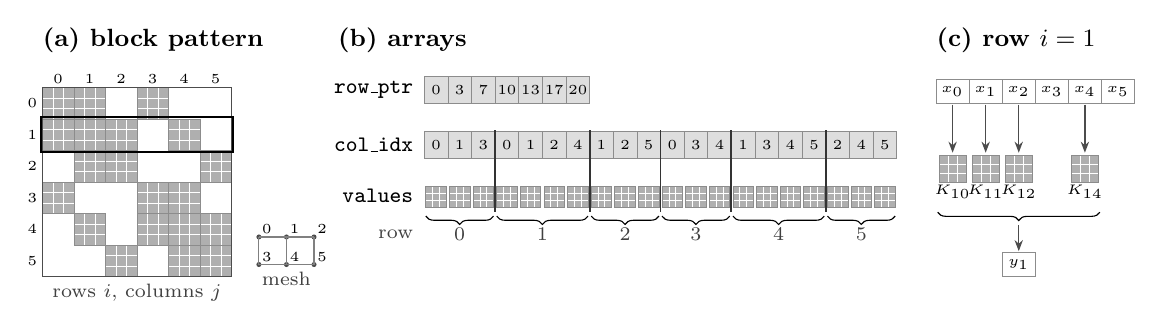
\begin{tikzpicture}
  % ---------------------------------------------------------------- (a) the matrix
  \def\s{0.4}
  \node[title] at (0, 3.3) {(a) block pattern};
  \foreach \i/\cols in {0/{0,1,3}, 1/{0,1,2,4}, 2/{1,2,5}, 3/{0,3,4}, 4/{1,3,4,5}, 5/{2,4,5}} {
    \foreach \j in \cols {
      \pgfmathsetmacro{\x}{\j*\s}\pgfmathsetmacro{\y}{(5-\i)*\s+0.3}
      \blk{\x}{\y}{\s}{cvalue!55}
    }
    \node[num, anchor=east] at (-0.06, {(5-\i)*\s+\s/2+0.3}) {$\i$};
    \node[num, anchor=south] at ({\i*\s+\s/2}, {6*\s+0.34}) {$\i$};
  }
  \draw[frame] (0,0.3) rectangle (6*\s, 6*\s+0.3);
  \draw[black, line width=0.8pt] (-0.02, 4*\s+0.3-0.02) rectangle (6*\s+0.02, 5*\s+0.3+0.02);
  \node[note, anchor=north] at (3*\s, 0.24) {rows $i$, columns $j$};
  % the mesh the pattern comes from
  \begin{scope}[shift={(2.75,0.45)}, scale=0.7]
    \foreach \a in {0,1,2} \foreach \b in {0,1} {
      \pgfmathtruncatemacro{\n}{(1-\b)*3+\a}
      \fill[black!70] (\a*0.5,\b*0.5) circle (1.3pt);
      \node[num, anchor=south west, inner sep=1pt] at (\a*0.5,\b*0.5) {$\n$};
    }
    \draw[black!50, line width=0.4pt] (0,0) -- (1,0) (0,0.5) -- (1,0.5) (0,0) -- (0,0.5) (0.5,0) -- (0.5,0.5) (1,0) -- (1,0.5);
    \node[note, anchor=north] at (0.5,-0.08) {mesh};
  \end{scope}

  % ---------------------------------------------------------------- (b) the arrays
  \begin{scope}[shift={(4.85,0)}]
    \def\w{0.3}
    \node[title] at (-1.1, 3.3) {(b) arrays};
    \node[lab, anchor=east] at (-0.1, 2.67) {\texttt{row\_ptr}};
    \foreach \v [count=\k from 0] in {0,3,7,10,13,17,20} {
      \cell{\k*\w}{2.5}{\w}{0.34}{cindex!50}
      \node[num] at ({\k*\w+\w/2}, 2.67) {$\v$};
    }
    \node[lab, anchor=east] at (-0.1, 1.97) {\texttt{col\_idx}};
    \node[lab, anchor=east] at (-0.1, 1.32) {\texttt{values}};
    \foreach \c [count=\k from 0] in {0,1,3, 0,1,2,4, 1,2,5, 0,3,4, 1,3,4,5, 2,4,5} {
      \cell{\k*\w}{1.8}{\w}{0.34}{cindex!50}
      \node[num] at ({\k*\w+\w/2}, 1.97) {$\c$};
      \blk{\k*\w+0.02}{1.18}{0.26}{cvalue!55}
    }
    \foreach \a/\b/\r in {0/3/0, 3/7/1, 7/10/2, 10/13/3, 13/17/4, 17/20/5} {
      \draw[brace] ({\b*\w-0.02}, 1.1) -- ({\a*\w+0.02}, 1.1) node[midway, below=4pt, note] {$\r$};
    }
    \node[note, anchor=east] at (-0.1, 0.83) {row};
    \foreach \b in {3,7,10,13,17} \draw[black!80, line width=0.7pt] ({\b*\w}, 1.12) -- ({\b*\w}, 2.16);
  \end{scope}

  % ---------------------------------------------------------------- (c) one row of the product
  \begin{scope}[shift={(11.35,0)}]
    \def\w{0.42}
    \node[title] at (0, 3.3) {(c) row $i = 1$};
    % x, one node per box
    \foreach \j in {0,...,5} {
      \cell{\j*\w}{2.5}{\w}{0.3}{white}
      \node[num] at ({\j*\w+\w/2}, 2.65) {$x_{\j}$};
    }
    % the row's blocks under their columns, x_j gathered
    \foreach \j in {0,1,2,4} {
      \blk{\j*\w+0.04}{1.5}{0.34}{cvalue!55}
      \draw[arr] ({\j*\w+\w/2}, 2.48) -- ({\j*\w+\w/2}, 1.87);
      \node[num, anchor=north] at ({\j*\w+\w/2}, 1.47) {$K_{1\j}$};
    }
    \draw[brace] (5*\w-0.02, 1.15) -- (0.02, 1.15);
    \draw[arr] (2.5*\w, 0.95) -- (2.5*\w, 0.62);
    \cell{2.5*\w-0.21}{0.3}{0.42}{0.3}{white}
    \node[num] at (2.5*\w, 0.45) {$y_1$};
  \end{scope}
\end{tikzpicture}
\end{document}
